%% This file explains the options available to you for editing the file
%% main.tex.

%% The commands in this file allow you to specify options such as
%% spacing, double-sided printing, a draft copy, etc.   By default, 12pt
%% and lgrind are included; lgrind is the 2e style for including code in
%% your thesis.

%% \documentclass[12pt]{mitthesis}
%% \usepackage{lgrind}
%% \pagestyle{plain}

%% You can add options in the documentclass line as follows:

%% 	o  singlespace
%% 	\documentclass[12pt,singlespace]{mitthesis}
	
%% 	o  twoside
%% 	\documentclass[12pt,twoside]{mitthesis}

%% 	o  draft   (make sure to change the pagestyle to drafthead as well)
%% 	\documentclass[12pt,draft]{mitthesis}
%% 	\usepackage{lgrind}
%% 	\pagestyle{drafthead}

%% 	o vi   (for course vi and course viii theses)
%% 	\documentclass[12pt,vi]{mitthesis}

%% Any options you would use for report.sty will work here as well.


%% You should not need to change the first three lines and last two lines
%% below.  Be sure to include an \include command for each file you are
%% including in your thesis.
  
%% % -*-latex-*-
% 
% For questions, comments, concerns or complaints:
% thesis@mit.edu
% 
%
% $Log: cover.tex,v $
% Revision 1.9  2019/08/06 14:18:15  cmalin
% Replaced sample content with non-specific text.
%
% Revision 1.8  2008/05/13 15:02:15  jdreed
% Degree month is June, not May.  Added note about prevdegrees.
% Arthur Smith's title updated
%
% Revision 1.7  2001/02/08 18:53:16  boojum
% changed some \newpages to \cleardoublepages
%
% Revision 1.6  1999/10/21 14:49:31  boojum
% changed comment referring to documentstyle
%
% Revision 1.5  1999/10/21 14:39:04  boojum
% *** empty log message ***
%
% Revision 1.4  1997/04/18  17:54:10  othomas
% added page numbers on abstract and cover, and made 1 abstract
% page the default rather than 2.  (anne hunter tells me this
% is the new institute standard.)
%
% Revision 1.4  1997/04/18  17:54:10  othomas
% added page numbers on abstract and cover, and made 1 abstract
% page the default rather than 2.  (anne hunter tells me this
% is the new institute standard.)
%
% Revision 1.3  93/05/17  17:06:29  starflt
% Added acknowledgements section (suggested by tompalka)
% 
% Revision 1.2  92/04/22  13:13:13  epeisach
% Fixes for 1991 course 6 requirements
% Phrase "and to grant others the right to do so" has been added to 
% permission clause
% Second copy of abstract is not counted as separate pages so numbering works
% out
% 
% Revision 1.1  92/04/22  13:08:20  epeisach

% NOTE:
% These templates make an effort to conform to the MIT Thesis specifications,
% however the specifications can change. We recommend that you verify the
% layout of your title page with your thesis advisor and/or the MIT 
% Libraries before printing your final copy.
\title{Towards Fully Decentralized Multiagent Trajectory Planning in Real-world Environments}

\author{Kota Kondo}
% If you wish to list your previous degrees on the cover page, use the 
% previous degrees command:
%       \prevdegrees{A.A., Harvard University (1985)}
% You can use the \\ command to list multiple previous degrees
%       \prevdegrees{B.S., University of California (1978) \\
%                    S.M., Massachusetts Institute of Technology (1981)}
\department{Department of Aeronautics and Astronautics}

% If the thesis is for two degrees simultaneously, list them both
% separated by \and like this:
% \degree{Doctor of Philosophy \and Master of Science}
\degree{Master of Science in Aeronautics and Astronautics}

% As of the 2007-08 academic year, valid degree months are September, 
% February, or June.  The default is June.
\degreemonth{June}
\degreeyear{2023}
\thesisdate{June 1, 2023}

%% By default, the thesis will be copyrighted to MIT.  If you need to copyright
%% the thesis to yourself, just specify the `vi' documentclass option.  If for
%% some reason you want to exactly specify the copyright notice text, you can
%% use the \copyrightnoticetext command.  
%\copyrightnoticetext{\copyright IBM, 1990.  Do not open till Xmas.}

% If there is more than one supervisor, use the \supervisor command
% once for each.
\supervisor{Jonathan P. How}{Richard C. Maclaurin Professor of Aeronautics and Astronautics}

% This is the department committee chairman, not the thesis committee
% chairman.  You should replace this with your Department's Committee
% Chairman.
\chairman{Arthur C. Chairman}{Chairman, Department Committee on Graduate Theses}

% Make the titlepage based on the above information.  If you need
% something special and can't use the standard form, you can specify
% the exact text of the titlepage yourself.  Put it in a titlepage
% environment and leave blank lines where you want vertical space.
% The spaces will be adjusted to fill the entire page.  The dotted
% lines for the signatures are made with the \signature command.
\maketitle

% The abstractpage environment sets up everything on the page except
% the text itself.  The title and other header material are put at the
% top of the page, and the supervisors are listed at the bottom.  A
% new page is begun both before and after.  Of course, an abstract may
% be more than one page itself.  If you need more control over the
% format of the page, you can use the abstract environment, which puts
% the word "Abstract" at the beginning and single spaces its text.

%% You can either \input (*not* \include) your abstract file, or you can put
%% the text of the abstract directly between the \begin{abstractpage} and
%% \end{abstractpage} commands.

% First copy: start a new page, and save the page number.
\cleardoublepage
% Uncomment the next line if you do NOT want a page number on your
% abstract and acknowledgments pages.
% \pagestyle{empty}
\setcounter{savepage}{\thepage}
\begin{abstractpage}
% $Log: abstract.tex,v $
% Revision 1.1  93/05/14  14:56:25  starflt
% Initial revision
% 
% Revision 1.1  90/05/04  10:41:01  lwvanels
% Initial revision
% 
%
%% The text of your abstract and nothing else (other than comments) goes here.
%% It will be single-spaced and the rest of the text that is supposed to go on
%% the abstract page will be generated by the abstractpage environment.  This
%% file should be \input (not \include 'd) from cover.tex.
Multiagent trajectory planning is a critical aspect of unmanned aerial vehicle (UAV) applications such as search and rescue missions, surveillance, and package delivery. However, developing a scalable and robust multiagent trajectory planner for UAVs poses significant challenges. Real-world deployments face difficulties such as communication delays and flying through dynamic environments, which can lead to undesired collisions.
\\

To address these challenges, we propose a decentralized, asynchronous multiagent trajectory planner called Robust MADER (RMADER). With centralized planners, each agent must listen to a single entity that plans all the trajectories, but this approach may lead to a single point of failure and depend heavily on communication with the central entity. In contrast, decentralized planners enable each agent to plan its own trajectory, making them inherently more scalable. Asynchronous planning allows each agent to trigger the planning step independently, without waiting at a synchronization barrier, making it more scalable than synchronous methods.
\\

However, decentralized, asynchronous multiagent trajectory planners are susceptible to communication delays, which could cause collisions. To overcome this issue, RMADER is designed to be robust to communication delays by introducing a delay-check step and a two-step trajectory-sharing scheme. RMADER guarantees safety by always keeping a collision-free trajectory and performing a delay check step, even under communication delay. 
\\

To evaluate RMADER, we performed extensive benchmark studies against state-of-the-art trajectory planners and flight experiments using a decentralized communication architecture called a mesh network with multiple UAVs in dynamic environments. The results demonstrate RMADER's robustness and capability to carry out collision avoidance in dynamic environments, outperforming existing state-of-the-art methods with a 100\% collision-free success rate.
\\

In summary, this thesis proposes a decentralized, asynchronous approach to multiagent trajectory planning approach for UAVs that is scalable and robust to communication delay. RMADER's promising results in both simulation and flight experiments contribute to the advancement of multiagent trajectory planning for UAVs.

\end{abstractpage}

% Additional copy: start a new page, and reset the page number.  This way,
% the second copy of the abstract is not counted as separate pages.
% Uncomment the next 6 lines if you need two copies of the abstract
% page.
% \setcounter{page}{\thesavepage}
% \begin{abstractpage}
% % $Log: abstract.tex,v $
% Revision 1.1  93/05/14  14:56:25  starflt
% Initial revision
% 
% Revision 1.1  90/05/04  10:41:01  lwvanels
% Initial revision
% 
%
%% The text of your abstract and nothing else (other than comments) goes here.
%% It will be single-spaced and the rest of the text that is supposed to go on
%% the abstract page will be generated by the abstractpage environment.  This
%% file should be \input (not \include 'd) from cover.tex.
Multiagent trajectory planning is a critical aspect of unmanned aerial vehicle (UAV) applications such as search and rescue missions, surveillance, and package delivery. However, developing a scalable and robust multiagent trajectory planner for UAVs poses significant challenges. Real-world deployments face difficulties such as communication delays and flying through dynamic environments, which can lead to undesired collisions.
\\

To address these challenges, we propose a decentralized, asynchronous multiagent trajectory planner called Robust MADER (RMADER). With centralized planners, each agent must listen to a single entity that plans all the trajectories, but this approach may lead to a single point of failure and depend heavily on communication with the central entity. In contrast, decentralized planners enable each agent to plan its own trajectory, making them inherently more scalable. Asynchronous planning allows each agent to trigger the planning step independently, without waiting at a synchronization barrier, making it more scalable than synchronous methods.
\\

However, decentralized, asynchronous multiagent trajectory planners are susceptible to communication delays, which could cause collisions. To overcome this issue, RMADER is designed to be robust to communication delays by introducing a delay-check step and a two-step trajectory-sharing scheme. RMADER guarantees safety by always keeping a collision-free trajectory and performing a delay check step, even under communication delay. 
\\

To evaluate RMADER, we performed extensive benchmark studies against state-of-the-art trajectory planners and flight experiments using a decentralized communication architecture called a mesh network with multiple UAVs in dynamic environments. The results demonstrate RMADER's robustness and capability to carry out collision avoidance in dynamic environments, outperforming existing state-of-the-art methods with a 100\% collision-free success rate.
\\

In summary, this thesis proposes a decentralized, asynchronous approach to multiagent trajectory planning approach for UAVs that is scalable and robust to communication delay. RMADER's promising results in both simulation and flight experiments contribute to the advancement of multiagent trajectory planning for UAVs.

% \end{abstractpage}

\cleardoublepage

\section*{Acknowledgments}

This is the acknowledgements section. You should replace this with your
own acknowledgements.

%%%%%%%%%%%%%%%%%%%%%%%%%%%%%%%%%%%%%%%%%%%%%%%%%%%%%%%%%%%%%%%%%%%%%%
% -*-latex-*-

%% \pagestyle{plain}
%%   % -*- Mode:TeX -*-
%% This file simply contains the commands that actually generate the table of
%% contents and lists of figures and tables.  You can omit any or all of
%% these files by simply taking out the appropriate command.  For more
%% information on these files, see appendix C.3.3 of the LaTeX manual. 
\tableofcontents
\newpage
\listoffigures
\newpage
\listoftables


%% %% This is an example first chapter.  You should put chapter/appendix that you
%% write into a separate file, and add a line \include{yourfilename} to
%% main.tex, where `yourfilename.tex' is the name of the chapter/appendix file.
%% You can process specific files by typing their names in at the 
%% \files=
%% prompt when you run the file main.tex through LaTeX.
\chapter{Introduction}

\section{Motivation}

Due to its wide range of applications, multiagent UAV trajectory planning has been extensively studied~\cite{peng2022obstacle, batra_decentralized_2022, ryou_cooperative_2022, vinod_safe_2022, kuwata_cooperative_2011}. 
In real-world deployments, every communication message between agents arrives with some extent of communication latency, and therefore it is essential that a trajectory planner is robust to both communication delays and dynamic environments. However, achieving robustness to both communication delays in multiagent trajectory planning is still an open question in the literature. 

\section{Literature Review}\label{sec:literature_review}

We first illustrate the categories of multiagent trajectory planning. Multiagent planners can be centralized~\cite{park_efficient_2020, sharon_conflict-based_2015, robinson_efficient_2018} (one machine plans every agent's trajectory) or decentralized \cite{tordesillas_mader_2022, zhou_ego-swarm_2020, lusk_distributed_2020} (each agent plans its own trajectory).
Decentralized planners are more scalable and robust to failures of the centralized machine. Despite these advantages, a decentralized scheme requires communication between the agents, and communication delays could potentially introduce failure in the trajectory deconfliction between the agents~\cite{gielis_critical_2022}. 
It is also worth noting that there are two layers of decentralization \textemdash decentralization on planning and decentralization on hardware architecture. Even if planner is decentralized in terms of planning, agents can still rely on centralized communication architecture, such as WiFi, and centralized localization, such as motion capture system. 

Multiagent planners can also be classified according to whether or not they are asynchronous. In an asynchronous setting, each agent independently triggers the planning step without considering the planning status of other agents. 
Asynchronous approaches do not require a synchronous mechanism among agents and are, therefore, more scalable than synchronous approaches.
They are, however, also more susceptible to communication delays since agents plan and execute trajectories independently. See Table \ref{tab:multiagent_category} for the aforementioned multiagent trajectory planner categorization.

\begin{table}[h]
    \renewcommand{\arraystretch}{2.5}
    \scriptsize
    \begin{centering}
    \caption{\centering Multiagent Trajectory Planner Category}
    \label{tab:multiagent_category}
    \resizebox{\columnwidth}{!}{
    \begin{tabular}{>{\centering\arraybackslash}m{0.05\columnwidth} >{\centering\arraybackslash}m{0.15\columnwidth} || >{\centering\arraybackslash}m{0.3\columnwidth} >{\centering\arraybackslash}m{0.3\columnwidth}}
    & & \ \ \ \ \ \ \ \tikzmark{a} & \ \ \ \ \ \ \ \ \ \ \ \ \ \ \ \ \ \ \ \ \ \ \ \ \ \ \ \ \ \ \ \tikzmark{b} \tabularnewline
    & & \textbf{Synchronous} & \textbf{Asynchronous} \tabularnewline
    \hline 
    \hline 
    \tikzmark{c} & \textbf{Centralized} & \cite{park_efficient_2020, sharon_conflict-based_2015, robinson_efficient_2018} & No methods proposed \tabularnewline
    \cline{2-4}
    \tikzmark{d} & \textbf{Decentralized} & \cite{chen_decoupled_2015, liu_towards_2018, park_online_2022, toumieh_decentralized_2022} & \cite{cap_asynchronous_2013, tordesillas_mader_2022, zhou_ego-swarm_2020, senbaslar_asynchronous_2022}, and \textbf{RMADER} \tabularnewline
    \end{tabular}}
    \par\end{centering}
    \begin{tikzpicture}[overlay, remember picture, shorten >=.5pt, shorten <=.5pt, transform canvas={yshift=.25\baselineskip}]
        \draw[thick, ->] ({pic cs:a}) -- ({pic cs:b}) node[midway, anchor=south] {\scriptsize Scalability};
        \draw[thick, ->] ({pic cs:c}) -- ({pic cs:d}) node[midway, fill=white] {\scriptsize Scalability};
    \end{tikzpicture}
\vspace*{0.5em}
\end{table}

Many decentralized state-of-the-art trajectory planners do not consider communication delays or explicitly state assumptions about communication. 
For example, \textbf{SCP}~\cite{chen_decoupled_2015}, \textbf{decNS}~\cite{liu_towards_2018}, and \textbf{LSC}~\cite{park_online_2022} are decentralized and synchronous, but SCP and decNS implicitly and LSC explicitly assume a perfect communication environment without any communication delays.

\newcommand{\NoRed}{\textbf{\textcolor{red}{No}}}
\newcommand{\YesGreen}{\textbf{\textcolor{ForestGreen}{Yes}}}

\begin{table}[!t]
    \renewcommand{\arraystretch}{1.2}
    \scriptsize
    \begin{centering}
    \caption{\centering State-of-the-art Decentralized Multiagent Planners}
    \label{tab:state_of_the_art_comparison}
    % \resizebox{1.0\columnwidth}{!}{
    \begin{tabular}{>{\centering\arraybackslash}m{0.3\columnwidth} >{\centering\arraybackslash}m{0.18\columnwidth} >{\centering\arraybackslash}m{0.2\columnwidth} >{\centering\arraybackslash}m{0.18\columnwidth}}
    \toprule 
    \textbf{Method} & \textbf{Asynchronous?} & \textbf{Robust to Comm. Delay?} & \textbf{Hardware in Dynamic Env.?}\tabularnewline
    \hline 
    \hline 
    \textbf{SCP}~\cite{chen_decoupled_2015}  & \multirow{3}[1]{*}{\NoRed{}} & \multirow{3}[1]{*}{\NoRed{}} & \multirow{3}[1]{*}{\NoRed{}} \tabularnewline
    \cline{0-0}
    \textbf{decNS}~\cite{liu_towards_2018} &&& \tabularnewline
    \cline{0-0}
    \textbf{LSC}~\cite{park_online_2022} &&& \tabularnewline
    \hline 
    \textbf{decMPC}~\cite{toumieh_decentralized_2022} & \NoRed{} & \YesGreen{} & \NoRed{} \tabularnewline
    \hline
    \textbf{EDG-Team}~\cite{hou_enhanced_2022} & \YesGreen{}/\NoRed{}\footnotemark[2] & \NoRed{} & \NoRed{} \tabularnewline
    \hline 
    \textbf{ADPP}~\cite{cap_asynchronous_2013} & \YesGreen{}\footnotemark[3] & \NoRed{} & \NoRed{} \tabularnewline
    \hline
    \textbf{MADER}~\cite{tordesillas_mader_2022} & \YesGreen{} & \NoRed{} & \NoRed{} \tabularnewline
    \hline 
    \textbf{EGO-Swarm}~\cite{zhou_ego-swarm_2020} & \YesGreen{} & \NoRed{} & \NoRed{} \tabularnewline
    \hline 
    \textbf{AsyncBVC}~\cite{senbaslar_asynchronous_2022} & \YesGreen{} & \YesGreen{}  & \NoRed{} \tabularnewline
    \hline
    \textbf{RMADER \ (proposed)} & \YesGreen{} & \YesGreen{} & \YesGreen{} \tabularnewline
    \bottomrule
    \end{tabular}
    % }
    \par\end{centering}
\vspace*{0.5em}
\footnotesize{$^2$ \!\!\! EDG-Team triggers joint optimization in dense environments and switches to a centralized, synchronous planner.} \\
\footnotesize{$^3$  \!\!\!\! Asynchronous but requires priority information for planning.}
\vspace{-2em}
\end{table}

The algorithm \textbf{decMPC}~\cite{toumieh_decentralized_2022} is decentralized, but it requires synchronicity and communication delays to be within a fixed planning period.
\textbf{EDG-Team}~\cite{hou_enhanced_2022} is a decentralized semi-asynchronous planner, which solves joint optimization as a group. 
EDG-Team cooperatively tackles the path-planning problem but implicitly assumes no communication delays. 
\textbf{ADPP}~\cite{cap_asynchronous_2013} is asynchronous\footnote{As in \cite{tordesillas_mader_2022}, we define asynchronous planning to be when the agent triggers trajectory planning independently without considering the planning status of other agents. 
However, ADPP~\cite{cap_asynchronous_2013} implements a prioritized asynchronous approach, meaning plannings are not fully independently triggered.} and decentralized, but it assumes perfect communication without delay. 
Our previous work \MADER{}~\cite{tordesillas_mader_2022} is asynchronous and decentralized but assumes no communication delays.
\textbf{EGO-Swarm}~\cite{zhou_ego-swarm_2020} also proposes a decentralized, asynchronous planner that requires agents to periodically broadcast a trajectory at a fixed frequency, and each agent immediately performs collision checks upon receiving the message. EGO-Swarm is the first fully decentralized, asynchronous trajectory planner successfully demonstrating hardware experiments, yet it still suffers from collisions due to communication delays, as shown in Section~\ref{sec:sim}. 
\textbf{AsyncBVC}~\cite{senbaslar_asynchronous_2022} proposes an asynchronous decentralized trajectory planner that can guarantee safety even with communication delays.
However, the future trajectories are constrained by past separating planes, which can overconstrain the solution space and hence increase conservatism.
In addition, it relies on discretization when solving the optimization problem, meaning that safety is only guaranteed on the discretization points. Additionally, AsyncBVC was only tested in simulations, so its applicability in real-world hardware is unclear. 
%In contrast, our approach instead is able to guarantee safety in a continuous approach by leveraging the MINVO basis~\cite{tordesillas_minvo_2022}.
For clarification, we define a dynamic environment as an environment with dynamic obstacles. The difference between an agent and an obstacle is that an agent can make decisions based on given information. An obstacle, on the other hand, simply follows a pre-determined trajectory regardless of what else is in the environment.

\section{Contributions}

To address robustness to communication delays in dynamic environments, we propose \textbf{Robust MADER} (\RMADER{}), a decentralized and asynchronous multiagent trajectory planner that is capable of generating collision-free trajectories in dynamic environments even in the presence of realistic communication delays.
As shown in Table~\ref{tab:state_of_the_art_comparison}, RMADER is the first approach to demonstrate trajectory planning in dynamic environments while maintaining robustness to communication delays. Our contributions include:
\begin{enumerate}
  \item An algorithm that guarantees collision-free trajectory generation even in the presence of real-world communication delays between vehicles. 
  \item Extensive simulations comparing our approach to state-of-the-art methods under communication delays that demonstrate a \textbf{100\% success rate} of collision-free trajectory generation (see Table~\ref{tab:sim_compare}).
  \item Theoretical analysis of collision-free guarantee on RMADER
  \item A mesh network implementation using six agents. 
  \item Two, four, and six agent hardware flight experiments on a mesh network with two dynamic obstacles, achieving \SI{5.8}{\m/\s}. Our work is the first to demonstrate a multiagent trajectory planner that is robust to communication delays with multiple dynamic obstacles in hardware.
\end{enumerate}

Chapter~\ref{} presents RMADER's trajectory deconfliction approach and theoretical guarantee. Chapter~\ref{} provides simulation results and benchmark studies, and Chapter~\ref{} showcases hardware experiment results, where RMADER's robustness to communication delays.

%% %% This is an example first chapter.  You should put chapter/appendix that you
%% write into a separate file, and add a line \include{yourfilename} to
%% main.tex, where `yourfilename.tex' is the name of the chapter/appendix file.
%% You can process specific files by typing their names in at the 
%% \files=
%% prompt when you run the file main.tex through LaTeX.
\chapter{Trajectory Deconfliction}

\section{Issues with Other State-of-the-art Approaches}

As described in Section~\ref{sec:literature_review}, existing methods either implicitly or explicitly assume perfect communication environments, and with the presence of communication latency, their approaches' collision-safety guarantee no longer holds. 
MADER~\cite{tordesillas_mader_2022} guarantees collision-free trajectories under ideal communication through the use of the planning stages shown in Fig.~\ref{fig:mader_deconfliction}.
% When there is no communication delay, safety can be guaranteed by using the approach presented in our previous work MADER~\cite{tordesillas_mader_2022} (see Fig.~\ref{fig:mader_deconfliction}).
An agent plans its initial trajectory during \OptimizationStep{} (\OStep{}), followed by \CheckStep{} (\CStep{}) to ensure its plan does not lead to a collision.
Finally, \RecheckStep{} (\RStep{}) is used to check if the agent received any trajectory updates from other agents during \CStep{} - if so, an agent starts over planning at \OStep{}.
Although MADER does not have explicit safety guarantees in the presence of communication delays, its trajectories are still collision free for cases 1 and 2 shown in Fig.~\ref{fig:mader_deconfliction}. However,  collisions may occur in cases 3 and 4 of Fig.~\ref{fig:mader_deconfliction}.
These four cases are summarized in Fig.~\ref{fig:mader_deconfliction} and Table~\ref{tab:safety_guarantees_delays}.

\begin{figure*}[t]
\centering
  \centering
  \resizebox{1.0\textwidth}{!}{%
    \begin{tikzpicture}
        [
        % define styles
        greenbox/.style={shape=rectangle, fill=opt_color, draw=black},
        bluebox/.style={shape=rectangle, fill=check_color, draw=black},
        redbox/.style={shape=rectangle, fill=recheck_color, draw=black},
        ]
        
        % coordinate
        \newcommand\Ay{5.5}
        \newcommand\Axo{3}
        \newcommand\Axc{8}
        \newcommand\Axr{10}
        \newcommand\Axe{11}
        
        \newcommand\By{2}
        \newcommand\Bxo{5}
        \newcommand\Bxc{12}
        \newcommand\Bxr{15}
        
        % MADER deconfliction 
        % Agent A
            \node[text=red] at (0.5,\Ay+0.2) {\scriptsize Agent A};
            % previous iter.
            \filldraw[fill=check_color, draw=black, opacity=0.2] (0,\Ay) rectangle (1.5,\Ay-1.0);
            \filldraw[fill=recheck_color, draw=black, opacity=0.2] (1.5,\Ay) rectangle (\Axo,\Ay-1.0);
            % current iter.
            \filldraw[thick, fill=opt_color, draw=black] (\Axo,\Ay) rectangle (\Axc,\Ay-1.0);
            \filldraw[thick, fill=check_color, draw=black] (\Axc, \Ay) rectangle (\Axr, \Ay-1.0);
            \filldraw[thick, fill=recheck_color, draw=black] (\Axr, \Ay) rectangle (\Axe, \Ay-1.0);
            % next iter.
            \filldraw[fill=opt_color, draw=black, opacity=0.2] (\Axe, \Ay) rectangle (\Axe+4.5, \Ay-1.0);
            \filldraw[fill=check_color, draw=black, opacity=0.2] (\Axe+4.5, \Ay) rectangle (\Axe+5.5, \Ay-1.0);
            \filldraw[fill=recheck_color, draw=black, opacity=0.2] (\Axe+5.5, \Ay) rectangle (\columnwidth, \Ay-1.0);
        % Agent B
            \node[text=blue] at (0.5,\By+0.2) {\scriptsize Agent B};
            % previous iter.
            \filldraw[fill=check_color, draw=black, opacity=0.2] (0,\By) rectangle (\Bxo-0.5,\By-1.0);
            \filldraw[fill=recheck_color, draw=black, opacity=0.2] (\Bxo-0.5,\By) rectangle (\Bxo,\By-1.0);
            % current iter.
            \filldraw[thick, fill=opt_color, draw=black] (\Bxo,\By) rectangle (\Bxc,\By-1.0);
            \filldraw[thick, fill=check_color, draw=black] (\Bxc, \By) rectangle (\Bxr, \By-1.0);
            \filldraw[thick, fill=recheck_color, draw=black] (\Bxr, \By) rectangle (\Bxr+1, \By-1.0);
            % next iter.
            \filldraw[fill=opt_color, draw=black, opacity=0.2] (\Bxr+1, \By) rectangle (\columnwidth, \By-1.0);

        \draw[thick, densely dotted] (\Axe,-0.0) -- (\Axe,\Ay-1.0) node[] at (\Axe, -0.3) {\tiny $t_{\trajA{}{}}^A$};
            
        % Axis
        \draw[thick,->] (0,0) -- (\columnwidth,0) node[anchor=north east] {time};
        
        % traj. msgs
        \draw[thick, ->, draw=red] (\Axe,\Ay-1.0) -- (\Axe,\Ay-2.2) node[midway,fill=white, text=red] {\tiny \trajA{}};
        \draw[thick, <-, draw=red] (\Bxc-0.3,\By) -- (\Bxc-0.3,\By+0.3) node[anchor=south,text=black] {\tiny case 1};
        \draw[thick, <-, draw=red] (\Bxc+0.5,\By) -- (\Bxc+0.5,\By+0.3) node[anchor=south,text=black] {\tiny case 2};
        \draw[thick, <-, draw=red] (\Bxr+0.1,\By) -- (\Bxr+0.1,\By+0.3) node[anchor=south,text=black] {\tiny case 3};
        \draw[thick, <-, draw=red] (\Bxr+2,\By) -- (\Bxr+2,\By+0.3) node[anchor=south,text=black] {\tiny case 4};
        
        % legend in the sequence
        \node[font=\bfseries,right] at (\Axo,\Ay-0.15) {\tiny Optimization (O\textsubscript{A})};
        \node[font=\bfseries,right] at (\Axc,\Ay-0.15) {\tiny Check (C\textsubscript{A})};
        \node[font=\bfseries,right] at (\Axr-0.47,\Ay+0.15) {\tiny Recheck (R\textsubscript{A})};

        \node[font=\bfseries,right] at (\Bxo,\By-0.15) {\tiny O\textsubscript{B}};
        \node[font=\bfseries,right] at (\Bxc,\By-0.15) {\tiny C\textsubscript{B}};
        \node[font=\bfseries,right] at (\Bxr,\By-0.15) {\tiny R\textsubscript{B}};
        
        % text
        \node[color=gray] at (1.0,\Ay-0.15) {\scriptsize Prev. iter.};
        \node[color=gray] at (0.95\columnwidth,\Ay-0.15) {\scriptsize Next iter.};
        \node[color=gray] at (1,\By-0.15) {\scriptsize Prev. iter.};
        \node[color=gray] at (0.95\columnwidth,\By-0.15) {\scriptsize Next iter.};
    \end{tikzpicture}
    }
    \vspace*{-5mm}
    \captionof{figure}{MADER deconfliction: \AgentA{} solves \OStepA{} to find its optimal trajectory, constrained by other agents' trajectories. \AgentA{} then begins \CStepA{} to determine if that generated trajectory has any conflicts with trajectories received during \OStepA{}. Finally, in \RStepA{}, \AgentA{} checks if it received any trajectories during \CStep{}. The four cases shown in the figure correspond to different communication delays, resulting in \trajA{} being received by \AgentB{} at different times. Designed to guarantee safety when there is no communication delays, MADER also guarantees safety when \trajA{} arrives during \OStepB{} (Case 1) or \CStepB{} (Case 2), but could cause collisions if \trajA{} is received during/after (Case 3/4) \RStepB{}.
    % MADER assumes no communication delay between Agents, but that can be too strong an assumption in the real world. In the case that communication delay occurs, \AgentB{} receives \trajA{} at $t^{ci}$ corresponding to Case i:
    % \begin{itemize}
    %     \item Case 1 \& 2: \AgentB{} can detect its trajectory conflicts with 
    %     \trajA{} during its \CStep{} and {\tt Recheck}, respectively.
    %     \item Case 3: MADER assumes Agents will not receive trajectories in {\tt Recheck}, which is short, but this could occur. In such a case it can not detect collisions.
    %     \item Case 4: \AgentB{} already published its trajectory after {\tt Recheck} and therefore cannot detect conflicts. 
    % \end{itemize}
    }
  \label{fig:mader_deconfliction}
\end{figure*}

\section{RMADER's trajectory deconfliction}

To achieve robustness to communication delays, we replace the \RecheckStep{} with \DelayCheckStep{} (\DCStep{}), where each agent repeatedly checks if its newly optimized trajectory conflicts with other agents' trajectories.
If an agent detects conflicts during \DCStep{}, it discards the new trajectory and starts another \OStep{} while executing its previous trajectory. 
If no collisions are detected in \DCStep{}, it starts executing the new trajectory. 
To guarantee collision-free trajectory generation, \DCStep{} needs to be longer than the possible longest communication delay (i.e., \NeccessaryCond{}). 
That way, an agent can always keep at least one collision-free trajectory. 
It could, however, not be ideal for introducing such a long \delayParameter{}, and therefore, in Section~\ref{sec:sim} we also tried $\delta_{\text{DC}}<\delta_{\text{max}}$ and measure its performance. 
Fig.~\ref{fig:rmader_deconfliction} shows how RMADER deals with communication delays.
Furthermore, Table~\ref{tab:safety_guarantees_delays} shows all the possible cases in which communication delays could occur and how these are handled by RMADER to generate collision-free trajectories even with communication delays.
The pseudocode of RMADER deconfliction is given in Algorithm~\ref{alg:rmader}. First, Agent~B runs \OStep{} to obtain \trajBNew{} and broadcasts it if \CStep{} is satisfied 
(Line~\ref{line:broadcast_traj_B_new}). This \CStep{} aims to determine if \trajBNew{} has any conflicts with trajectories received in \OStep{}. Then, Agent~B commits either \trajBPrev{} or \trajBNew{} - if \DCStep{} detects conflicts, Agent~B commits to \trajBPrev{} (Line~\ref{line:DC_not_satisfied}), and if \DCStep{} detects no conflicts, \trajBNew{} (Line~\ref{line:DC_satisfied}). This committed trajectory is then broadcast to the other agents (Line~\ref{line:broadcast_traj_B}). Table~\ref{tab:mader_vs_rmader} highlights the differences between MADER and RMADER.

\begin{figure*}[t]
\centering
  \resizebox{1.0\textwidth}{!}{%
       \begin{tikzpicture}
       [
        % define styles
        greenbox/.style={shape=rectangle, fill=opt_color, draw=black},
        bluebox/.style={shape=rectangle, fill=check_color, draw=black},
         yellowbox/.style={shape=rectangle, fill=delaycheck_color, draw=black},
        ]
        
        % coordinate
        \newcommand\Ay{5.5}
        \newcommand\Axo{3}
        \newcommand\Axc{8}
        \newcommand\Axr{10}
        \newcommand\Axe{11}
        
        \newcommand\By{2}
        \newcommand\Bxo{5}
        \newcommand\Bxc{12}
        \newcommand\Bxr{15}
        \newcommand\Bxe{17}
        
        % RMADER deconfliction 
        % Agent A
            \node[text=red] at (0.5,\Ay+0.2) {\scriptsize Agent A};
            % previous iter.
            \filldraw[fill=check_color, draw=black, opacity=0.2] (0,\Ay) rectangle (1.5,\Ay-1.0);
            \filldraw[fill=delaycheck_color, draw=black, opacity=0.2] (0.5,\Ay) rectangle (\Axo,\Ay-1.0);
            % current iter.
            \filldraw[thick, fill=opt_color, draw=black] (\Axo,\Ay) rectangle (\Axc,\Ay-1.0);
            \filldraw[thick, fill=check_color, draw=black] (\Axc, \Ay) rectangle (\Axr, \Ay-1.0);
            \filldraw[thick, fill=delaycheck_color, draw=black] (\Axr, \Ay) rectangle (\Axe, \Ay-1.0);
            % next iter.
            \filldraw[fill=opt_color, draw=black, opacity=0.2] (\Axe, \Ay) rectangle (\Axe+1.5, \Ay-1.0);
            \filldraw[fill=check_color, draw=black, opacity=0.2] (\Axe+1.5, \Ay) rectangle (\columnwidth, \Ay-1.0);
        % Agent B
            \node[text=blue] at (0.5,\By+0.2) {\scriptsize Agent B};
            % previous iter.
            \filldraw[fill=check_color, draw=black, opacity=0.2] (0,\By) rectangle (\Bxo-0.5,\By-1.0);
            \filldraw[fill=delaycheck_color, draw=black, opacity=0.2] (\Bxo-0.5,\By) rectangle (\Bxo,\By-1.0);
            % current iter.
            \filldraw[thick, fill=opt_color, draw=black] (\Bxo,\By) rectangle (\Bxc,\By-1.0);
            \filldraw[thick, fill=check_color, draw=black] (\Bxc, \By) rectangle (\Bxr, \By-1.0);
            \filldraw[thick, fill=delaycheck_color, draw=black] (\Bxr, \By) rectangle (\Bxe, \By-1.0);
            % next iter.
            \filldraw[fill=opt_color, draw=black, opacity=0.2] (\Bxe, \By) rectangle (\columnwidth, \By-1.0);
            % \filldraw[fill=check_color, draw=black, opacity=0.2] (\Bxe+1.0, \By) rectangle (\columnwidth-1, \By-1.0);
        
        % time label
        % \draw[thick, densely dotted] (\Axo,0) -- (\Axo,\Ay-1.0) node[] at (\Axo, -0.25) {\tiny $t_o^A$};
        %\draw[thick, densely dotted] (\Axc,0) -- (\Axc,\Ay-1.0) node[] at (\Axc, -0.25) {\tiny $t_c^A$};
        \draw[thick, densely dotted] (\Axr,0) -- (\Axr,\Ay-1.0) node[] at (\Axr, -0.25) {\tiny t\textsubscript{traj\textsubscript{A\textsubscript{new}}}};
        \draw[thick, densely dotted] (\Axe,0) -- (\Axe,\Ay-1.0) node[] at (\Axe, -0.25) {\tiny t\textsubscript{traj\textsubscript{A}}};
            
        % Axis
        \draw[thick,->] (0,0) -- (\columnwidth,0) node[anchor=north east] {time};
        
        % traj. msgs
        \draw[thick, ->, draw=red] (\Axr,\Ay-1.0) -- (\Axr,\Ay-2.2) node[midway,fill=white, text=red] {\tiny \trajANew{}};
        \draw[thick, ->, draw=red] (\Axe,\Ay-1.0) -- (\Axe,\Ay-2.2) node[midway,fill=white, text=red] {\tiny \trajA{}};
        \draw[thick, <-, draw=red] (\Bxc-0.2,\By) -- (\Bxc-0.2,\By+0.3)  node[anchor=south,text=black] {\tiny case 1};
        \draw[thick, <-, draw=red] (\Bxc+0.6,\By) -- (\Bxc+0.6,\By+0.3) node[anchor=south,text=black] {\tiny case 2};
        \draw[thick, <-, draw=red] (\Bxr+0.4,\By) -- (\Bxr+0.4,\By+0.3) node[anchor=south,text=black] {\tiny case 3};
        \draw[thick, <-, draw=red] (\Bxe+0.4,\By) -- (\Bxe+0.4,\By+0.3) node[anchor=south,text=black] {\tiny case 4};
        
        % legend in the sequence
        \node[font=\bfseries,right] at (\Axo,\Ay-0.15) {\tiny O\textsubscript{A}};
        \node[font=\bfseries,right] at (\Axc,\Ay-0.15) {\tiny C\textsubscript{A}};
        \node[font=\bfseries,right] at (\Axr,\Ay-0.15) {\tiny DC\textsubscript{A}};

        \node[font=\bfseries,right] at (\Bxo,\By-0.15) {\tiny O\textsubscript{B}};
        \node[font=\bfseries,right] at (\Bxc,\By-0.15) {\tiny C\textsubscript{B}};
        \node[font=\bfseries,right] at (\Bxr,\By-0.15) {\tiny DC\textsubscript{B}};
        
        % legend box
        % \matrix [draw,below left] at (current bounding box.north east) {
        % \matrix [draw,below left,fill=white,opacity=1.0] at (15, \Ay) {
        %   \node [greenbox,label=right:Optimization] {}; \\
        %   \node [bluebox,label=right:Check] {}; \\
        %   \node [redbox,label=right:Recheck] {}; \\
        % };
        
        % text
        \node[color=gray] at (1,\Ay-0.15) {\scriptsize Prev. iter.};
        \node[color=gray] at (0.95\columnwidth,\Ay-0.15) {\scriptsize Next iter.};
        \node[color=gray] at (1,\By-0.15) {\scriptsize Prev. iter.};
        \node[color=gray] at (\columnwidth,\By-1.45) {\scriptsize Next iter.};
        
    \end{tikzpicture}
    }
    
  \captionof{figure}{RMADER deconfliction: After \CStepA{}, \AgentA{} keeps executing the trajectory from the previous iteration, \trajAPrev{}, while checking potential collisions of newly optimized trajectory, \trajANew{}. 
  This is because \trajANew{} might have conflicts due to communication delays and need to be checked in \DCStepA{}, and traj\textsubscript{A\textsubscript{prev}} is ensured to be collision-free. If collisions are detected in either \CStepA{} or \DCStepA{}, \AgentA{} keeps executing \trajAPrev{} (i.e., $\text{\trajA{}}\leftarrow \text{\trajAPrev{}}$). If \DCStepA{} does not detect collisions, \AgentA{} broadcasts and starts implementing \trajANew{} (i.e., $\text{\trajA{}}\leftarrow \text{\trajANew{}}$).}
  \label{fig:rmader_deconfliction}
\end{figure*}

In MADER~\cite{tordesillas_mader_2022} and RMADER, UAVs plan trajectories asynchronously and broadcast the results to each other.  Each agent uses these trajectories as constraints in the optimization problem. Assuming no communication delays exist, safety can be guaranteed using our previous approach presented in MADER (summarized in Section~\ref{subsec:mader_deconfliction}). 
This safety guarantee, however, breaks when an agent's planned trajectory is received by other agents with some latency. Section~\ref{subsec:rmader_deconfliction} shows how RMADER guarantees safety even with communication delays. We use the definitions shown in Table~\ref{tab:delaydefinitions}.

\begin{table}[b]
    \vspace{-1.5em}
    \begin{centering}
    \caption{Definitions of the different delay quantities: Note that, by definition, $0\le\delayIntroduced\le\delayActual{}\le\delayActualMax{}$. See also Figs~\ref{fig:sim_actual_comm_delay} and~\ref{fig:comm_delay_on_centr} for the actual histogram of the delays in simulation and hardware, respectively.  }
    \renewcommand{\arraystretch}{2}
    \begin{centering}
    \begin{tabular}{>{\centering\arraybackslash}m{0.1\columnwidth} >{\arraybackslash}m{0.7\columnwidth}}
    \toprule 
    \delayActual{} & Actual communication delays among agents. \tabularnewline
    \hline 
    \delayActualMax{} & \makecell[l]{Possible maximum communication delay. } \tabularnewline
    \hline 
    \delayIntroduced{} & \makecell[l]{Introduced communication delay in simulations. } \tabularnewline
    \hline 
    \delayParameter{} & \makecell[l]{Length of \DelayCheckStep{} in RMADER. \\ To guarantee safety, $\delayActualMax{}\le\delayParameter{}$ must be satisfied.} \tabularnewline
    \bottomrule
    \end{tabular}
    \par\end{centering}
    \label{tab:delaydefinitions}
    \par\end{centering}
\end{table}

\begin{table}
\caption{Safety guarantees under communication delays: Depending on when \trajA{} is received by Agent B, the deconfliction takes place at different stages. MADER does not guarantee safety if \trajA{} is received during \RStepB{} or during the following iteration, while RMADER guarantees safety in all the cases. Note that in RMADER, if Agent~B does not receive \trajA{} by the end of \DCStepB{}, then the deconfliction is performed by Agent A (specifically, in \CStepA{} or \DCStepA{}) and not by Agent B. Agent A will use \trajBNew{} and/or \trajB{} for this.}
\label{tab:safety_guarantees_delays}
\begin{centering}
\renewcommand{\arraystretch}{1.2}
\resizebox{1.0\columnwidth}{!}{
\setlength\extrarowheight{0.3em}
\begin{tabular}{>{\centering}m{0.3\columnwidth} || >{\centering}m{0.2\columnwidth} >{\centering}m{0.2\columnwidth} >{\centering}m{0.2\columnwidth} >{\centering}m{0.2\columnwidth}}
\toprule
\multicolumn{1}{>{\centering}m{0.1\columnwidth}||}{} & \multicolumn{4}{c}{\textbf{MADER}} \tabularnewline[0.2em]
\hline
\textbf{When \trajA{} received}  & \makecell{\OStepB{} \\ (Case 1)} & \makecell{\CStepB{} \\ (Case 2)} & \makecell{\RStepB{} \\ (Case 3)} & \makecell{\textbf{Next iter.} \\ (Case 4)} \tabularnewline[0.4em]
\hline 
\textbf{\trajA{} deconflicted? When?} & \makecell{\YesGreen{} \\ \CStepB{}}  & \makecell{\YesGreen{} \\ \RStepB{}}  & \NoRed{}  & \NoRed{} \tabularnewline
\bottomrule
\end{tabular}
}
%\hfill
\vspace{0.2cm}

\resizebox{1.0\columnwidth}{!}{
\setlength\extrarowheight{0.3em}
\begin{tabular}{>{\centering}m{0.3\columnwidth} || >{\centering}m{0.2\columnwidth} >{\centering}m{0.2\columnwidth} >{\centering}m{0.2\columnwidth} >{\centering}m{0.2\columnwidth}}
\toprule
\multicolumn{1}{>{\centering}m{0.1\columnwidth}||}{} & \multicolumn{4}{c}{\textbf{RMADER}}\tabularnewline[0.2em]
\hline
\textbf{When \trajANew{}/\trajA{} received}  & \makecell{\OStepB{} \\ (Case 1)} & \makecell{\CStepB{} \\ (Case 2)} & \makecell{\DCStepB{} \\ (Case 3)} & \makecell{\textbf{Next iter.} \\ (Case 4)} \tabularnewline
\hline 
\textbf{\trajANew{}/\trajA{} deconflicted? When?} & \makecell{\YesGreen{} \\ \CStepB{}} & \makecell{\YesGreen{} \\ \DCStepB{}}  & \makecell{\YesGreen{} \\ \DCStepB{}}  & \makecell{\YesGreen{} \\ \CStepA{} or \DCStepA{}} \tabularnewline
\bottomrule
\end{tabular}
}

\par\end{centering}
\end{table}

\begin{algorithm}
    \begin{algorithmic}[1]
    \Require traj\textsubscript{B}, a feasible trajectory
    \While{not goal reached}
        \State \trajBNew{} $=$ \textproc{\OptimizationStep{}()} \label{line:traj_opt}
        \If{\textproc{\CheckStep}(\trajBNew{}) $==$ False} 
            \State Go to Line 2
        \EndIf
        \State Broadcast \trajBNew{} \label{line:broadcast_traj_B_new}
        \If{\textproc{\DelayCheckStep{}}(\trajBNew{}) $==$ False} 
            \State \trajB{} $\leftarrow$ \trajBPrev{}, and go to Line~\ref{line:broadcast_traj_B}\label{line:DC_not_satisfied}
        \EndIf
        \State \trajB{} $\leftarrow$ \trajBNew{} \label{line:DC_satisfied}
        \State Broadcast \trajB{} \label{line:broadcast_traj_B}
    \EndWhile
    \end{algorithmic}
    \caption{Robust MADER - Agent B}
    \label{alg:rmader}
\end{algorithm}

\begin{table}
\begin{centering}
\caption{\centering Differences between MADER and RMADER}
\label{tab:mader_vs_rmader}
\renewcommand{\arraystretch}{1.1}
\resizebox{1.0\columnwidth}{!}{
\scriptsize
\begin{tabular}{>{\centering\arraybackslash}m{0.4\columnwidth} >{\centering\arraybackslash}m{0.4\columnwidth}}
\toprule
\textbf{MADER} & \textbf{RMADER}\tabularnewline
\hline 
\hline 
Upon successful \CStep{} and \RStep{}, the newly optimized trajectory is broadcast to other agents 
%Broadcast only the committed trajectory. This committed trajectory will be newly optimized trajectory if both \CStep{} and \RStep{} are satisfied, and the previous trajectory
& Upon successful \CStep{}, \trajJNew{} is broadcast. After \DCStep{}, the committed trajectory \trajJ{} (which is either \trajJNew{} and \trajJPrev{} depending on whether \DCStep{} is satisfied or not) is broadcast \tabularnewline
\hline 
\RStep{} is a Boolean check to see if the agent received traj.
in \CStep{} & \DCStep{} is a sequence of collision checks\tabularnewline
\hline 
\RStep{} is very short & \DCStep{} lasts \delayParameter{} seconds\tabularnewline
\bottomrule
\end{tabular}
}
\par\end{centering}
\vspace{-2em}
\end{table}

\begin{algorithm}
    \newcommand{\algorithmicbreak}{\textbf{break}}
    \begin{algorithmic}[1] %1 means every 1 line the line will be numbered
    \Function {\textproc{\DelayCheckStep{}}}{\trajBNew{}}
        \For {\delayParameter{} seconds}
            \If{\trajBNew{} collides with any trajectory in $\mathcal{Q}_B$}    
                %\State Discards \trajB{}
                \State \Return False
             \EndIf
         \EndFor
    \State \Return True
    \EndFunction
    \end{algorithmic}
    \caption{Delay Check - Agent B}\label{alg:pess_delaycheck}
\end{algorithm}

\newcommand{\QB}{\ensuremath{\mathcal{Q}_B}}

Agent~B stores the trajectories received from other agents in a set \QB{}; for example, for each Agent~J, Agent~B will store the committed trajectory of Agent~J, \trajJ{}, and possibly the newly optimized trajectory \trajJNew{} if any new committed trajectory has still not been broadcast. Figure~\ref{fig:QB_definition} shows the way Agent B stores trajectories from Agent A. 
\QB{} is used in \OStep{}, \CheckStep{}, and \DCStep{},  where Agent~B checks for collision against all the trajectories stored in \QB{}. Note that \QB{} is updated in parallel with \OStep{} and \DCStep{}. 
At the beginning of \OStepB{}, an agent generates an optimal trajectory, \trajBNew{}, using all the trajectories stored in \QB{} as constraints, and then, Agent B checks for \trajBNew{}'s potential collisions against \QB{}, which is updated in optimization. 
Finally, Agent~B repeatedly checks for collisions against \QB{} in \DCStepB{}, which lasts for \delayParameter{}. 
Note that \CStep{} is not necessary to guarantee safety in RMADER - \OStep{} followed by \DCStep{} alone can generate collision-free trajectories as long as \NeccessaryCond{} holds. Though \CStep{} detects collisions before broadcasting any (possibly conflicted) trajectories and allows an agent to start another \OStep{}, which prevents unnecessary communication.

\begin{figure}
    \centering
    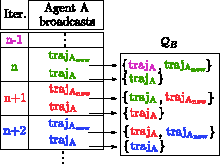
\includegraphics[width=0.6\columnwidth]{figures/QB_definition.pdf}
    \setlength{\belowcaptionskip}{-0.5em}
    \caption{Agent~B stores in \QB{} the last committed trajectory of Agent~A. It will also contain the newly optimized trajectory \trajANew{} while the new committed trajectory has still not been received by Agent~B. }
    \label{fig:QB_definition}
\end{figure}

Now we provide a theoretical analysis of RMADER's trajectory deconfliction. 
First, we introduce Lemma~\ref{lem:two_agent_suffices_multiagent}, which allows us to scale up and apply two-agent deconfliction analysis to multiagent deconfliction, and then Proposition~\ref{prop:rmader_deconfliction_theorem} provides a theoretical guarantee of RMADER's deconfliction approach. 

\newtheorem{lemma}{Lemma}
\begin{lemma}
\label{lem:two_agent_suffices_multiagent}
In decentralized asynchronous trajectory planning, collision safety guarantee between any two agents is a sufficient condition for multiagent collision safety guarantee. 
\end{lemma}

\begin{proof}
Decentralized asynchronous multiagent trajectory deconfliction is a set of two-agent trajectory deconfliction, and therefore in case of trajectory deconfliction is guaranteed between every pair of any two agents, multiagent trajectory deconfliction is also guaranteed. 
\end{proof}

\newtheorem{prop}{Proposition}
\begin{prop}
\label{prop:rmader_deconfliction_theorem}
Given $\delayParameter{}>\delayActualMax{}$, RMADER is guaranteed to be collision-free under communication delay.
\end{prop}

\begin{proof}
By Lemma~\ref{lem:two_agent_suffices_multiagent}, to prove RMADER's multiagent collision-free guarantee, we show RMADER's collision-free guarantee between two agents.
Note that in case the decentralized asynchronous planner uses hard constraints, such as RMADER, as long as at any given time, at least one of the two agents has knowledge of the other agent's trajectory, collision safety is guaranteed between the two agents \textemdash In RMADER, this condition is implied by $\delayParameter{}>\delayActualMax{}$. 
To prove RMADER's collision-free guarantee, we thoroughly go through all the possible 12 cases of trajectory deconfliction between two agents - One agent sends its trajectory to the other agent's either \OStep{}, \CStep{}, or \DCStep{}, and the other agent can receive this trajectory in either \OStep{}, \CStep{}, \DCStep{}, or the next iteration. 
For clarity, we define the time \AgentA{} publishes its newly optimized trajectory as \tApub, the time \AgentB{} receives it as \tBrec, and Agent B's \OptimizationStep/\CheckStep/\DelayCheckStep{} as \OStepB/\CStepB/\DCStepB, respectively. All the possible cases are illustrated in Table~\ref{tab:rmader_possible_cases}; for example, case 3 denotes \AgentA{} publishes in \OStepB{}, and \AgentB{} receives it in \DCStepB{}. Note that cases 1-4 correspond to cases 1-4 in Fig.~\ref{fig:rmader_deconfliction}.
\begin{table}[H]
\caption{\centering RMADER Trajectory Deconfliction Cases}
\label{tab:rmader_possible_cases}
\begin{centering}
\renewcommand{\arraystretch}{1.2}
\resizebox{1.0\columnwidth}{!}{
\begin{tabular}{ c c || c c c c }
\toprule
 & & \multicolumn{4}{c}{\tBrec}\tabularnewline
\cline{3-6} 
 & & \OStepB{} & \CStepB{} & \DCStepB{} & Next Iter. \tabularnewline
\hline \hline
\multirow{3}[1]{*}{\tApub} & \OStepB{} & case 1 & case 2 & case 3 & case 4 \tabularnewline
\cline{2-6} 
 & \CStepB{} & case 5 & case 6 & case 7 & case 8 \tabularnewline
\cline{2-6}
 & \DCStepB{} & case 9 & case 10 & case 11 & case 12 \tabularnewline
\bottomrule
\end{tabular}}
\par\end{centering}
\end{table}

\begin{itemize}
\item In Case 1, Agent B detects possible collisions in its \CStep{} before committing to any trajectory.
\item In Case 2, Agent B detects possible collisions in its \DCStep{} before committing to any trajectory.
\item In Case 3, Agent B detects possible collisions in its \DCStep{} before committing to any trajectory.
\item In Case 4, Given $\delayParameter{}>\delayActualMax{}$, this case will never occur.
\item Case 5 will never occur since \CStep{} comes after \OStep{}.
\item In Case 6, Agent B detects possible collisions in its \DCStep{} before committing to any trajectory.
\item In Case 7, Agent B detects possible collisions in its \DCStep{} before committing to any trajectory.
\item Case 8 will never occur because $\delayParameter{}>\delayActualMax{}$.
\item Case 9 will never occur since \DCStep{} comes after \OStep{}.
\item Case 10 will never occur since \DCStep{} comes after \CStep{}.
\item In Case 11, Agent B detects possible collisions in its \DCStep{} before committing to any trajectory.
\item In Case 12, Agent B will commit its trajectory at the end of its \DCStep{}, not knowing Agent A's potentially collision-prone trajectory. However, by $\delayParameter{}>\delayActualMax{}$, Agent B's newly optimized trajectory is published in either Agent A's \OStep{} or \CStep{}, and therefore, Agent A can detect potential collisions before committing to its trajectory.
\end{itemize}

As shown above, in all the possible cases, either one of the two can detect possible collisions. Therefore RMADER is guaranteed to be collision-free as long as $\delayParameter{}>\delayActualMax{}$ holds.
\end{proof}

\section{RMADER without Check}

As demonstrated in Algorithm~\ref{alg:pess_delaycheck}, \DCStep{} repeatedly executes \CheckStep{}, and therefore we can guarantee safety without \CheckStep{} as long as \DCStep{} is longer than \delayActualMax{}. However, this could increase the number of rejections of newly optimized trajectory because it is published before it is checked for potential collisions with trajectories received in \OStep, leading to more conservative results.
Note that even if we skip \CheckStep{} and publish \trajNew{}, \trajNew{} is not committed yet, and therefore, collision-free guarantee is ensured. Fig.~\ref{fig:wo_check_rmader_deconfliction} illustrates this scheme's trajectory deconfliction: 
\begin{itemize}
    \item Case 1 \& 2: \AgentB{} can detect its trajectory conflicts in \DCStepB.
    \item Case 3: As long as $\delayParameter{}>\delayActualMax{}$, Case 3 will not happen.
\end{itemize}

\begin{figure}[h]
\centering
  \centering
  \resizebox{1.0\textwidth}{!}{%
       \begin{tikzpicture}
       [
        % define styles
        greenbox/.style={shape=rectangle, fill=opt_color, draw=black},
        bluebox/.style={shape=rectangle, fill=check_color, draw=black},
         yellowbox/.style={shape=rectangle, fill=delaycheck_color, draw=black},
        ]
        
        % coordinate
        % coordinate
        \newcommand\Ay{5.5}
        \newcommand\Axo{3}
        \newcommand\Axc{8}
        \newcommand\Axr{10}
        \newcommand\Axe{11}
        
        \newcommand\By{2}
        \newcommand\Bxo{5}
        \newcommand\Bxc{12}
        \newcommand\Bxr{15}
        \newcommand\Bxe{17}
        
        % RMADER deconfliction 
        % Agent A
            \node[text=red] at (0.5,\Ay+0.2) {\scriptsize Agent A};
            % previous iter.
            \filldraw[fill=delaycheck_color, draw=black, opacity=0.2] (0,\Ay) rectangle (\Axo,\Ay-1.0);
            % current iter.
            \filldraw[thick, fill=opt_color, draw=black] (\Axo,\Ay) rectangle (\Axr,\Ay-1.0);
            \filldraw[thick, fill=delaycheck_color, draw=black] (\Axr, \Ay) rectangle (\Axe, \Ay-1.0);
            % next iter.
            \filldraw[fill=opt_color, draw=black, opacity=0.2] (\Axe, \Ay) rectangle (\Axe+2.5, \Ay-1.0);
            \filldraw[fill=delaycheck_color, draw=black, opacity=0.2] (\Axe+2.5, \Ay) rectangle (\columnwidth, \Ay-1.0);
        % Agent B
            \node[text=blue] at (0.5,\By+0.2) {\scriptsize Agent B};
            % previous iter.
            \filldraw[fill=opt_color, draw=black, opacity=0.2] (0,\By) rectangle (0.5,\By-1.0);
            \filldraw[fill=delaycheck_color, draw=black, opacity=0.2] (0.5,\By) rectangle (\Bxo,\By-1.0);
            % current iter.
            \filldraw[thick, fill=opt_color, draw=black] (\Bxo,\By) rectangle (\Bxc,\By-1.0);
            \filldraw[thick, fill=delaycheck_color, draw=black] (\Bxc, \By) rectangle (\Bxc+1.5, \By-1.0);
            % next iter.
            \filldraw[fill=opt_color, draw=black, opacity=0.2] (\Bxc+1.5, \By) rectangle (\columnwidth, \By-1.0);
        
        % time label
        % \draw[thick, densely dotted] (\Axo,0) -- (\Axo,\Ay-1.0) node[] at (\Axo, -0.25) {\tiny $t_o^A$};
        %\draw[thick, densely dotted] (\Axc,0) -- (\Axc,\Ay-1.0) node[] at (\Axc, -0.25) {\tiny $t_c^A$};
        \draw[thick, densely dotted] (\Axr,0) -- (\Axr,\Ay-1.0) node[] at (\Axr, -0.25) {\tiny t\textsubscript{traj\textsubscript{A\textsubscript{new}}}};
        \draw[thick, densely dotted] (\Axe,0) -- (\Axe,\Ay-1.0) node[] at (\Axe, -0.25) {\tiny t\textsubscript{traj\textsubscript{A}}};
        %\draw[thick, densely dotted] (\Bxc-0.2,\By) -- (\Bxc-0.2,-0.5) node[] at (\Bxc-0.2, -0.7) {\tiny $t^{c1}$};
        %\draw[thick, densely dotted]  (\Bxc+0.35,\By) -- (\Bxc+0.35,0) node[] at (\Bxc+0.35, -0.25) {\tiny $t^{c2}$};
        %\draw[thick, densely dotted] (\Bxr+0.4,\By) -- (\Bxr+0.4,0) node[] at (\Bxr+0.4, -0.25) {\tiny $t^{c3}$};
        %\draw[thick, densely dotted] (\Bxe+0.4,\By) -- (\Bxe+0.4,0) node[] at (\Bxe+0.4, -0.25) {\tiny $t^{c4}$};
            
        % Axis
        \draw[thick,->] (0,0) -- (\columnwidth,0) node[anchor=north east] {time};
        
        % traj. msgs
        \draw[thick, ->, draw=red] (\Axr,\Ay-1.0) -- (\Axr,\Ay-2.2) node[midway,fill=white, text=red] {\tiny \trajANew{}};
        \draw[thick, ->, draw=red] (\Axe,\Ay-1.0) -- (\Axe,\Ay-2.2) node[midway,fill=white, text=red] {\tiny \trajA{}};
        \draw[thick, <-, draw=red] (\Bxc-0.2,\By) -- (\Bxc-0.2,\By+0.3)  node[anchor=south,text=black] {\tiny case 1};
        \draw[thick, <-, draw=red] (\Bxc+0.6,\By) -- (\Bxc+0.6,\By+0.3) node[anchor=south,text=black] {\tiny case 2};
        \draw[thick, <-, draw=red] (\Bxr+0.4,\By) -- (\Bxr+0.4,\By+0.3) node[anchor=south,text=black] {\tiny case 3};
        
        % legend in the sequence
        \node[font=\bfseries,right] at (\Axo,\Ay-0.15) {\tiny O\textsubscript{A}};
        \node[font=\bfseries,right] at (\Axr,\Ay-0.15) {\tiny DC\textsubscript{A}};

        \node[font=\bfseries,right] at (\Bxo,\By-0.15) {\tiny O\textsubscript{B}};
        \node[font=\bfseries,right] at (\Bxc,\By-0.15) {\tiny DC\textsubscript{B}};
        
        % text
        \node[color=gray] at (1,\Ay-0.15) {\scriptsize Prev. iter.};
        \node[color=gray] at (0.95\columnwidth,\Ay-0.15) {\scriptsize Next iter.};
        \node[color=gray] at (1,\By-0.15) {\scriptsize Prev. iter.};
        \node[color=gray] at (0.95\columnwidth,\By-0.15) {\scriptsize Next iter.};
        
    \end{tikzpicture}
    }
    
  \captionof{figure}{RMADER deconfliction without \CheckStep{}: After \OStepA, \AgentA{} publishes its newly optimized trajectory \trajANew, while it keeps executing the trajectory from the previous iteration, traj\textsubscript{A\textsubscript{prev}}. As with Fig.~\ref{fig:rmader_deconfliction}, the agent checks conflicts \DCStepA{}, and if collisions are detected in \DCStepA{}, \AgentA{} continues on executing \trajAPrev{} (i.e., $\text{\trajA{}}\leftarrow \text{\trajAPrev{}}$). In case \DCStepA{} does not detect collisions, \AgentA{} broadcasts and starts implementing \trajANew{} (i.e., $\text{\trajA{}}\leftarrow \text{\trajANew{}}$).}
  \label{fig:wo_check_rmader_deconfliction}
\end{figure}

\section{Delay Check variations}

There are several ways to implement \DelayCheckStep{} depending on communication environments, and this section illustrates these variations.


\textbf{How the deconfliction is solved:} We can have two approaches:
\begin{itemize}
    \item \underline{Optimistic} (Algorithm~\ref{alg:opt_delaycheck}): It uses the ``first commits, first occupies" policy: An Agent A checks collisions only against the received trajectories that were generated before its own trajectory. If the received trajectory was generated after A's trajectory, Agent A does not need to be checked for collision because the other Agents will do that. 
    \item \underline{Pessimistic} (Algorithm~\ref{alg:pess_delaycheck}): An Agent checks for collisions using all the received trajectories, regardless of their timestamps. 

\end{itemize}

Both approaches guarantee safety as long as \NeccessaryCond{} holds for all the Agents. When \NeccessaryCond{} does not hold, neither approach can guarantee safety; however, {\tt Pessimistic} approach is more likely to avoid conflicts.

\subsubsection{Optimistic vs Pessimistic}

    Although this could generate conservative trajectories, Agents can avoid unnecessary collisions.
        As all the Agents follow this policy,  An Agent first checks if other Agents committed their trajectories earlier. If the Agent committed earlier, it would not check collisions since it is confident that the other Agents will eventually receive the Agent's trajectory during their {\tt Delay Check} and deconflict accordingly

One way to check conflicts in Delay Check is using the "first commits, first occupies" policy, which we call {\tt Optimistic Delay Check}. An Agent first checks if other Agents committed their trajectories earlier. If the Agent committed earlier, it would not check collisions since it is confident that the other Agents will eventually receive the Agent's trajectory during their {\tt Delay Check} and deconflict accordingly. 
Algorithm \ref{alg:opt_delaycheck} illustrates this approach. Note that {\tt Optimistic Delay Check} could lead to collisions in case the other UAVs' Delay Check is not long enough - though if \NeccessaryCond{} holds for all the Agents, 
all the Agents' {\tt Delay Check} is longer than the maximum communication delay, 
{\tt Optimistic Delay Check} guarantees safety. 
However, when obstacles are in flight space, {\tt Optimistic Delay Check} cannot guarantee safety since obstacles do not actively deconflict. 

As discussed above, {\tt Optimistic Delay Check} allows an Agent to commit trajectory even if the Agent detects collision as long as it has a priority. Yet, in case $\delayParameter\le\delayActual$ this overly optimistic approach could lead to collisions.

In {\tt Pessimistic Delay Check}, an Agent will not check the timestamp of other Agents' trajectory and only checks conflicts. Although this could generate conservative trajectories, Agents can avoid unnecessary collisions. {\tt Pessimistic Delay Check} is the one we use for all the simulations and hardware experiments of this paper.

Note that as long as \NeccessaryCond{} holds, both {\tt Optimistic} and {\tt Pessimistic Delay Check} guarantee collision safety, and in case \NeccessaryCond{} does not hold, neither approach can guarantee safety; however, {\tt Pessimistic} approach is more likely to avoid conflicts. Algorithm \ref{alg:opt_delaycheck} and \ref{alg:pess_delaycheck} provide details for {\tt Optimistic} and {\tt Pessimistic Delay Check}, respectively.


\footnotetext{Existing works suggest various methods to break the tie. Some works use Agents' pre-assigned ID; however, this could introduce other external information such as ID. We compared the x, y, and z axes in shared coordination, which is already shared as a part of trajectory in RMADER, and whichever has a higher value on the prioritized axis wins (we prioritize the x, y, and z axis in order). That way, Agents no longer need external information to break the tie.}

See Alg.~\ref{alg:opt_delaycheck}
\begin{algorithm}
    \newcommand{\algorithmicbreak}{\textbf{break}}
    traj\textsubscript{i} is another Agent's traj.\\
    timestamp\textsubscript{i} is a time when Agent i generated traj\textsubscript{i}
    \begin{algorithmic}[1] %1 means every 1 line the line will be numbered
    \Function {OptimisticDelayCheck}{\trajA{}}
        %\While {Elapsed time $<$ \delayParameter{}}
        \For {\delayParameter{} seconds}
            \If{timestamp\textsubscript{i} $<$ timestamp\textsubscript{A}}
                \If{\trajA{} collides with traj\textsubscript{i}}    
                    \State Discard \trajA{}
                    \State \algorithmicbreak
                \ElsIf{timestamp\textsubscript{i} $==$ timestamp\textsubscript{A}}
                    \State Tie Breaking\footnotemark
    %             \EndIf
    %         \EndIf
    %     \EndWhile
    % \EndFunction
    \end{algorithmic}
    \caption{Optimistic Delay Check - Agent A}\label{alg:opt_delaycheck}
\end{algorithm}

\begin{figure}
    \centering
    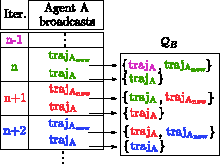
\includegraphics[width=0.6\columnwidth]{figures/QB_definition.pdf}
    \setlength{\belowcaptionskip}{-0.5em}
    \caption{Agent~B stores in \QB{} the last committed trajectory of Agent~A. It will also contain the newly optimized trajectory \trajANew{} while the new committed trajectory has still not been received by Agent~B. }
    \label{fig:QB_definition}
\end{figure}
%% \appendix
%% \chapter{Tables}

\begin{table}
\caption{Armadillos}
\label{arm:table}
\begin{center}
\begin{tabular}{||l|l||}\hline
Armadillos & are \\\hline
our	   & friends \\\hline
\end{tabular}
\end{center}
\end{table}

\clearpage
\newpage

%% \chapter{Figures}

\vspace*{-3in}

\begin{figure}
\vspace{2.4in}
\caption{Armadillo slaying lawyer.}
\label{arm:fig1}
\end{figure}
\clearpage
\newpage

\begin{figure}
\vspace{2.4in}
\caption{Armadillo eradicating national debt.}
\label{arm:fig2}
\end{figure}
\clearpage
\newpage

%% %% This defines the bibliography file (main.bib) and the bibliography style.
%% If you want to create a bibliography file by hand, change the contents of
%% this file to a `thebibliography' environment.  For more information 
%% see section 4.3 of the LaTeX manual.
\begin{singlespace}
\bibliography{main}
\bibliographystyle{plain}
\end{singlespace}

%% \end{document}

%% Comment: to include appendices use a single \appendix command followed 
%% by a number of \include{} commands as many files as needed, each of 
%% which should contain a \chapter{} command for the appendix title.
